% ============================================================
% BLOC 1: CONTEXT I PROBLEMA  (diapositives 1–4)
% ============================================================

% ---  DIAPOSITIVA 1 — Portada  ---
\begin{frame}[plain]
  \begin{center}
    \vspace{0.5cm}
    {\huge \bfseries \textcolor{upcblue}{Web Core View}}\\[0.25em]
    {\small \textcolor{gray}{Plataforma web integral per a la configuració, manteniment}\\
    \textcolor{gray}{i visualització de sistemes de videovigilància IP}}\\[0.8em]
    {\large \textit{Modernització de la interfície web d'un NVR professional}}\\[1.2em]

    {\large \textbf{Jan Rosell Caba}}\\[0.3em]
    {\small \textit{Director:} Fernando Gallego \quad|\quad \textit{Ponent:} Carles Farré}\\[0.2em]
    {\small Juny 2026}\\[1.5em]

    
\includegraphics[height=1.2cm]{../figures/logos/upc_complet.png}\hspace{0.8cm}
    
\includegraphics[height=1.2cm]{../figures/logos/fib_complet.png}\hspace{0.8cm}
    
\includegraphics[height=1.2cm]{../figures/logos/lanaccess_complet.png}
  \end{center}

  \note{
    Bon dia a tothom. El meu nom és Jan Rosell i avui presentaré el meu Treball de Fi de Grau: \textit{Web Core View}. Un projecte d'arquitectura web i modernització tecnològica per als gravadors de videovigilància professionals de Lanaccess.

    Tenim 20 minuts, així que aneu molt enrere, que la presentació serà dinàmica. Acabaré amb una demostració en vídeo de 5 minuts del sistema funcionant en viu.
  }
\end{frame}

% ---  DIAPOSITIVA 2 — Lanaccess i els NVR  ---
\begin{frame}{Lanaccess i els Gravadors NVR}
  \begin{columns}[T]
    \begin{column}{0.52\textwidth}
      \textbf{L'empresa}
      \begin{itemize}
        \item Lanaccess Telecom, SA: videovigilància professional.
        \item Producte estrella: família de gravadors \textbf{NXT}.
        \item Clients: empreses, institucions públiques, infraestructura crítica.
      \end{itemize}

      \vspace{0.5em}
      \textbf{El dispositiu}
      \begin{itemize}
        \item Fins a \textbf{152 càmeres} per unitat.
        \item SoC ARM (NXP i.MX), Linux Yocto.
        \item Desplegament \textit{standalone}: \textbf{sense Internet}.
      \end{itemize}
    \end{column}

    \begin{column}{0.44\textwidth}
      \begin{center}
        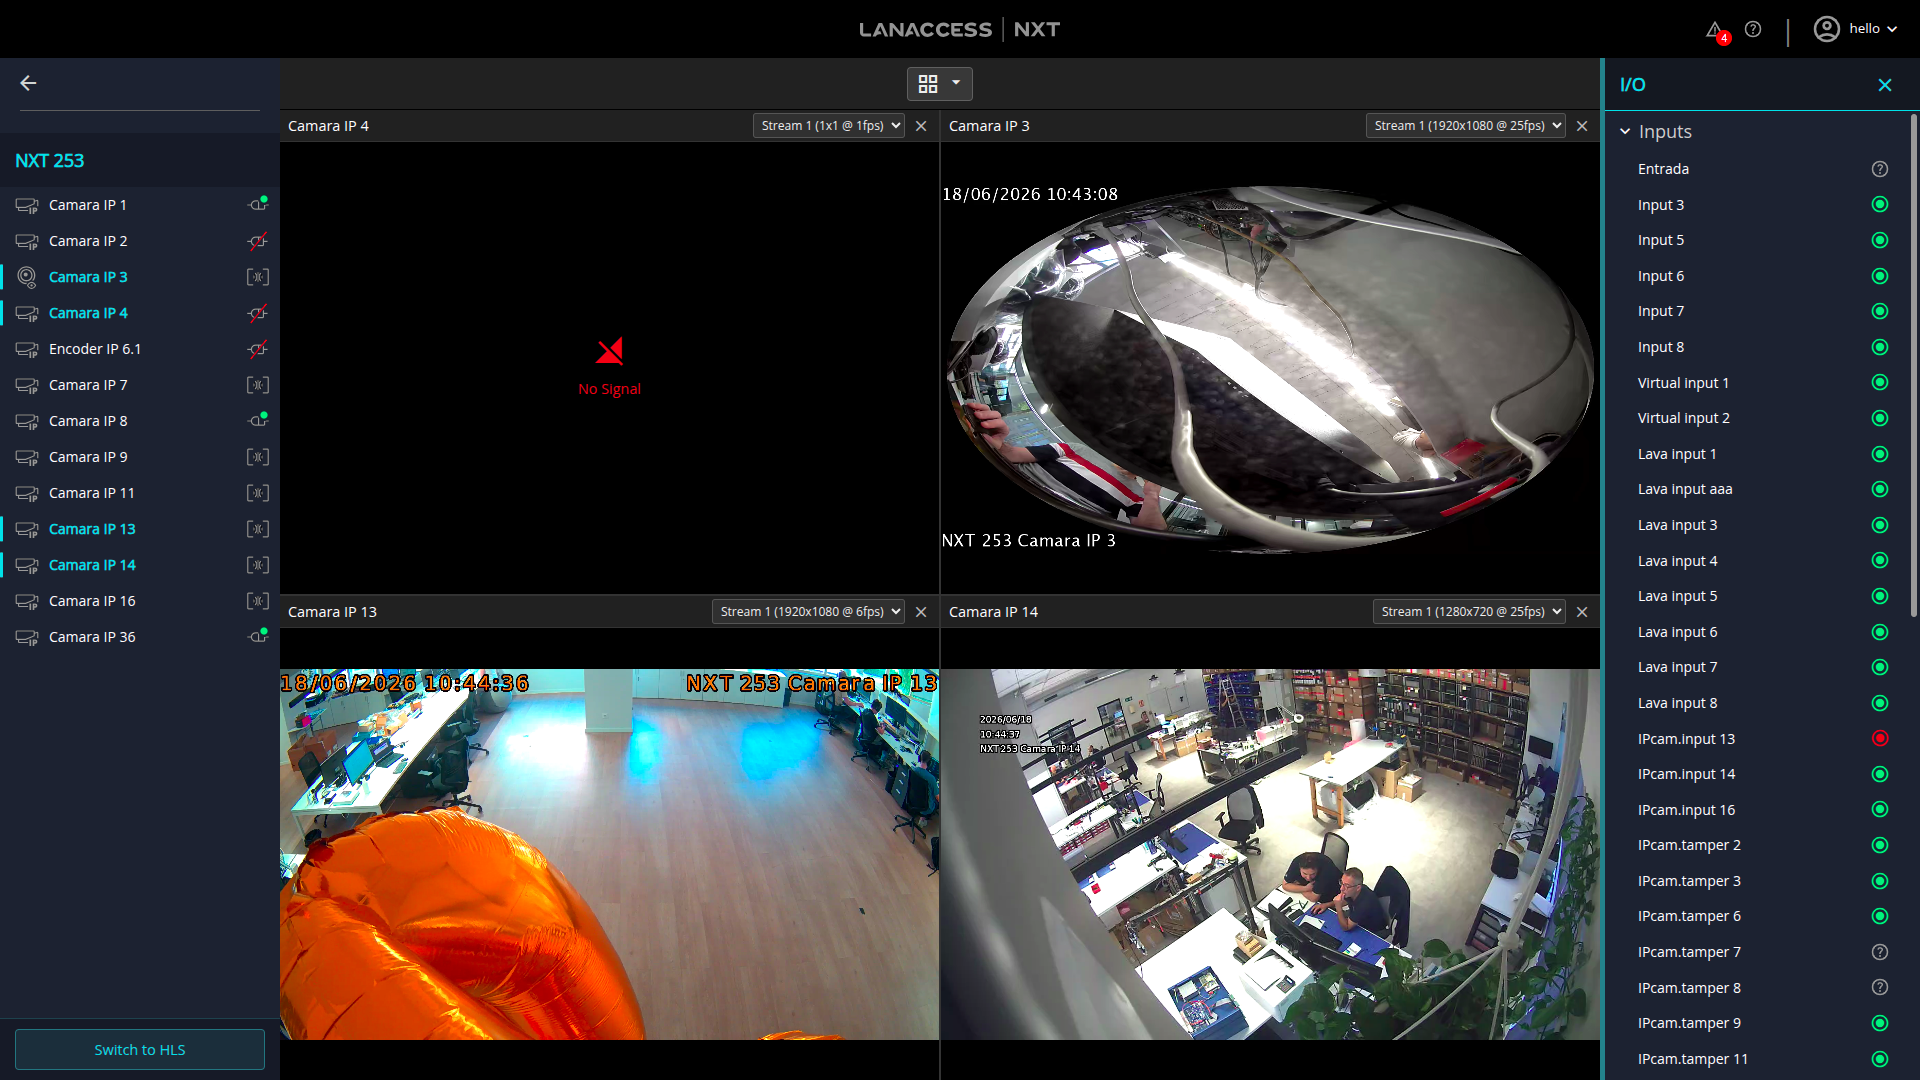
\includegraphics[width=\textwidth,keepaspectratio]{../figures/interficies/cameras.png}
      \end{center}
    \end{column}
  \end{columns}

  \note{
    Lanaccess és una empresa especialitzada en seguretat electrònica i videovigilància professional. El seu producte de referència és la família de gravadors NVR \textit{NXT}: dispositius que graven fins a 152 càmeres simultàniament. Funcionen sobre un processador ARM de NXP, corren Linux Yocto, i s'instal·len a les xarxes dels clients, que sovint no tenen sortida a Internet.

    Aquí hi ha la paraula clau: \textit{standalone}. Tot ha de funcionar sense dependre d'un servidor extern ni del núvol. L'NVR és l'únic servidor disponible.
  }
\end{frame}

% ---  DIAPOSITIVA 3 — El Problema: Fi d'una Era  ---
\begin{frame}{El Problema: La Fi d'una Era}
  \begin{columns}[T]
    \begin{column}{0.55\textwidth}
      \begin{alertblock}{L'herència: ActiveX (anys 90)}
        \begin{itemize}
          \item Plag dependent d'\textbf{Internet Explorer 11}.
          \item Microsoft tanca IE el \textbf{Juny 2022}.
          \item Incompatible amb macOS, Linux i mòbils.
          \item Vectors de seguretat documentats (OWASP).
        \end{itemize}
      \end{alertblock}

      \vspace{0.5em}
      \begin{itemize}
        \item Interfície estàtica: \textbf{sense reactivitat} ni temps real.
        \item Cada versió de firmware requeria canvis al frontend.
      \end{itemize}
    \end{column}

    \begin{column}{0.40\textwidth}
      \begin{block}{La pressió del mercat}
        \small Clients exigien accés des de qualsevol navegador i dispositiu modern.
      \end{block}

      \vspace{0.8em}
      \begin{block}{L'amenaça competitiva}
        \small Competidors amb interfícies web natives guanyaven terreny al catàleg NXT.
      \end{block}
    \end{column}
  \end{columns}

  \note{
    La situació de partida era crítica. Lanaccess tenia una plataforma web construïda als anys 90 basada en tecnologia ActiveX de Microsoft. El problema és que Internet Explorer 11, l'únic navegador que suportava ActiveX, va arribar al final de la seva vida el juny del 2022. I amb ell, va morir qualsevol possibilitat d'accedir als gravadors NXT des d'un Mac, un Linux, un mòbil, o simplement des de Chrome.

    A més, l'arquitectura era rígida: si el firmware canviava un paràmetre de configuració, un enginyer havia de modificar el frontend manualment. Això generava un deute tècnic creixent i una velocitat d'iteració molt lenta.

    La pressió del mercat era clara: els clients demandaven accés web modern, i la competència ja l'oferia.
  }
\end{frame}

% ---  DIAPOSITIVA 4 — L'Objectiu: Equip Autònom  ---
\begin{frame}{L'Objectiu: Un Sistema Web Autònom}

  \begin{center}
    \begin{tikzpicture}
      \node[draw=upcblue, rounded corners, fill=upclight, minimum width=2.5cm, minimum height=1.2cm, align=center] (browser) at (0,0) {\textbf{Navegador}\\\small Chrome/Firefox/Safari};
      \node[draw=upcblue, rounded corners, fill=upclight, minimum width=2.5cm, minimum height=1.2cm, align=center] (nvr) at (6,0) {\textbf{NVR NXT}\\\small Serveix tot};
      \draw[->, thick, upcblue] (browser.east) -- node[above]{\small HTTPS/WSS/WebRTC} (nvr.west);
    \end{tikzpicture}
  \end{center}

  \vspace{0.3em}
  \begin{columns}[T]
    \begin{column}{0.3\textwidth}
      \begin{exampleblock}{100\% Web}
        Cap plugin, cap instal·lació de client.
      \end{exampleblock}
    \end{column}
    \begin{column}{0.3\textwidth}
      \begin{exampleblock}{Autònom}
        L'NVR serveix l'app i el vídeo. Sense núvol.
      \end{exampleblock}
    \end{column}
    \begin{column}{0.3\textwidth}
      \begin{exampleblock}{Escalable}
        Nous firmwares no requereixen canvis al frontend.
      \end{exampleblock}
    \end{column}
  \end{columns}

  \note{
    L'objectiu del projecte es pot resumir en una frase: construir una aplicació 100\% web, basada en Angular 19, que s'executi de forma autònoma dins del propi gravador NVR, sense dependre de cap servidor extern ni plugin.

    Quan un operador obre el navegador i escriu la IP del gravador, l'NVR li serveix l'aplicació Angular, li ofereix els streams de vídeo i li envia les alarmes en temps real. Tot des del mateix dispositiu.

    I hi havia un tercer requisit diferencial: que l'aplicació fos escalable. Que si demà surten nous models de firmware amb noves opcions, el frontend s'adapti sol, sense que cap enginyer de software hagi de tocar el codi de la web.
  }
\end{frame}
